\section{Un approccio diverso}
Il nostro approccio si basa, come l'originale, sul trovare tutte le curve nei range di parametri prestabiliti per ogni pixel dell'immagine.\par
Quindi, a differenza del metodo visto prima, non andiamo a limitare la ricerca delle curve in qualche dimensione. Tuttavia cerchiamo di dimostrare come, nella maggior parte dei casi, sia più sensato identificare le curve in base alla posizione del loro centro rispetto agli altri due parametri.\par
Questo lo facciamo utilizzando una matrice di coordinate $(c,\ b)$ in cui salviamo le informazioni relative ai parametri $(a \text{ e } d)$ ed il numero di occorrenze che tale curva, la migliore, ha nel punto.\par
Com'è possibile osservare nello \hyperref[lst:ostinelli]{pseudocodice} a pagina seguente, alla riga 31 e seguenti, i dati (parametri della curva e occorrenze) vengono salvati solo nel caso in cui non ci sia stata una curva, precedentemente testata, che ha fatto un risultato migliore in termini di occorrenze in quel punto.\par
Questo ridurre le dimensioni del tensore a due (le coordinate del pixel) ci permette, oltre il notevole risparmio di spazio all'interno della memoria, di rappresentare il risultato della trasformata all'interno di un grafico tridimensionale, esattamente come nella trasformata lineare.\par
Gli assi del grafico sono $x$ e $y$ per le coordinate dei pixel e $z$ per le occorrenze.\par
Per un umano è estremamente intuitivo, a questo punto, identificare il centro della curva. Anche il sistema però è in grado, con uno sforzo computazionale ridotto, di trovare il massimo locale.\par
Rimane il problema della soglia critica, da scegliere in base al tipo di applicazione che vogliamo fare dell'algoritmo, che è intrinseco a questo tipo di trasformate.\par
Nella prossima sezione, analizzeremo qualche esempio. Per ognuno di questo abbiamo a disposizione quattro visualizzazioni che riescono a rendere un'idea del grafico tridimensionale:
\begin{enumerate}[itemsep=0pt, topsep=0pt]
    \item una isometrica, che permette di vedere il picco tridimensionale;
    \item una da sotto, utile grazie al colore, per vedere il centro della curva;
    \item vista dall'asse $X$;
    \item vista dall'asse $Y$.
\end{enumerate}

\newpage
\lstinputlisting[
    style=matlabStyle,
    caption={Pseudocodice per la trasformata in 2+1 dimensioni},
    label={lst:ostinelli}
]{codici/Ostinelli.m}
\newpage

\subsection{Analisi degli esempi}
Nel \hyperref[fig:sintentica_ostinelli_1]{primo esempio}, vediamo un picco al centro del grafico che segnala la presenza del centro della curva. Nella visione dall'asse $x$, è possibile notare come ci siano due pendii ai lati del picco.\par
Questo è dovuto alla lunghezza degli asintoti: alcune delle curve centrate nello stesso punto e con parametro $d$ (ampiezza) identico ma con parametro della curva $a$ diverso avranno in comune quella serie di punti.\par
Di conseguenza, la stessa curva, presente nel \hyperref[fig:sintentica_ostinelli_2]{secondo esempio}, che tuttavia ha gli asintoti tagliati, avrà un picco maggiormente isolato senza lasciarsi la scia sui versanti.\par
Nel \hyperref[fig:sintentica_ostinelli_3]{terzo} e \hyperref[fig:sintentica_ostinelli_4]{quarto esempio}, è possibile notare come sia precisa la posizione di identificazione. Con una forma, apprezzabile dalle visualizzazioni ortogonali agli assi $x$ ed $y$, molto simile a quello del \hyperref[fig:sintentica_ostinelli_2]{secondo esempio}.\par
Il \hyperref[fig:sintentica_ostinelli_5]{quinto esempio} dimostra come, in questo tipo di trasformata, dove i parametri della curva vanno in secondo piano rispetto alla presenza o meno della stessa, la sigmoide presente viene segnalata ma non è apprezzabile una significativa differenza per la parte inerente ai parametri $a$ e $d$.\par
Un caso decisamente interessante è il \hyperref[fig:sintentica_ostinelli_6]{sesto esempio} che, grazie alla presenza di due curve, palesa un fatto interessante.\par
I picchi dei relativi centri sono assolutamente ben visibili, di conseguenza ben individuabili anche grazie ad una soglia critica impostabile.\par
Da notare qualche picco più piccolo, ben visibile dall'asse $x$, anomalo. Questo è dovuto alla presenza, nello stesso grafico, di tutti i test delle possibili curve di parametri $a$ e $d$. Di conseguenza, vengono generate curve che intersecano le due presenti nell'immagine come si vede nell'\hyperref[fig:sovrapposizione]{immagine sotto}.\par
Infatti, la curva tratteggiata, potrebbe non essere presente ma essere rilevata in quanto alcuni punti andranno a votare proprio per quella.

\begin{figure}[h]
    \label{fig:sovrapposizione}
    \centering
    \fbox{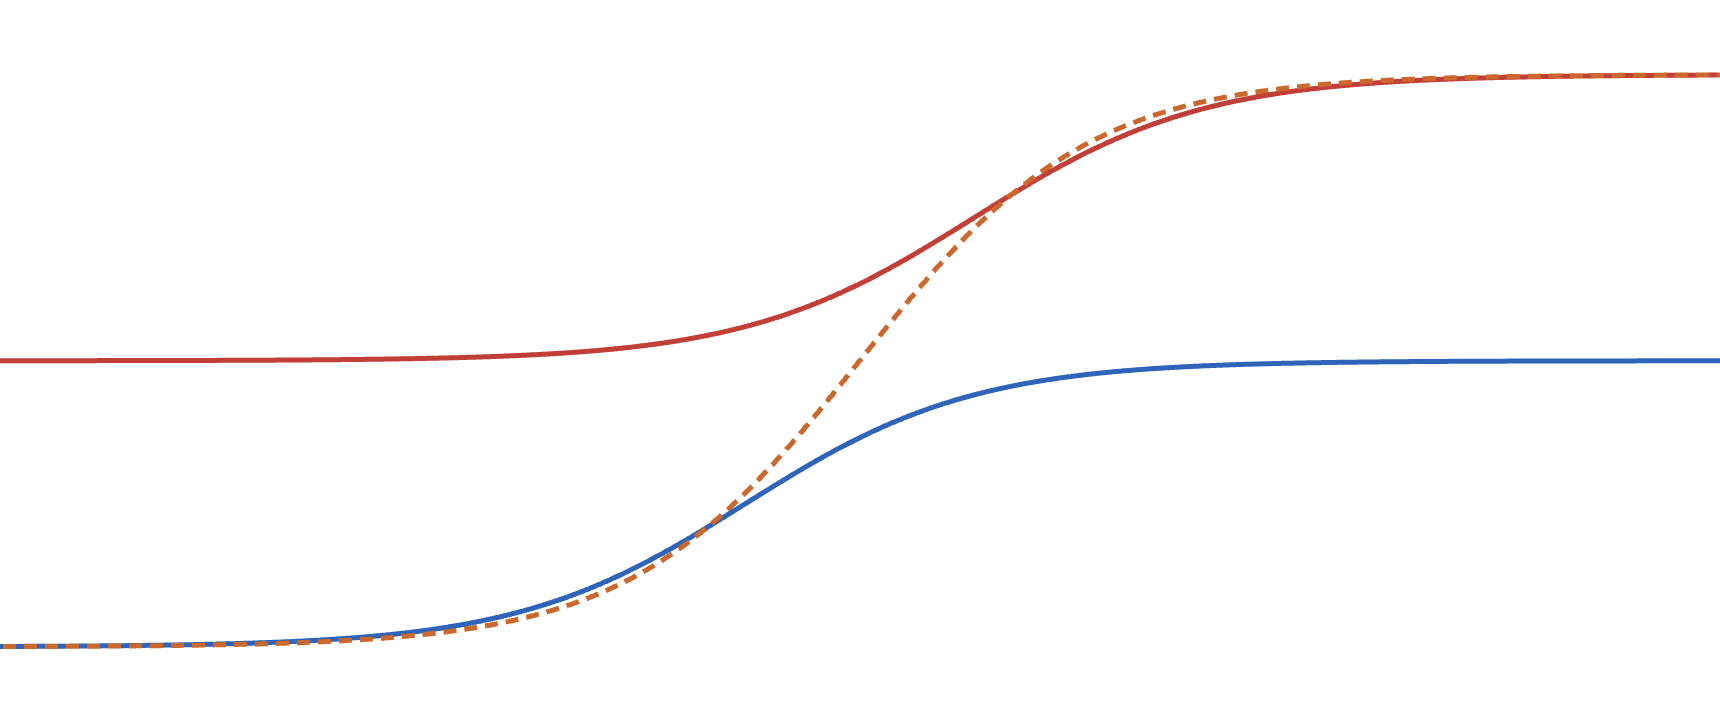
\includegraphics[width=0.71\textwidth]{immagini/altro/sovrapposizione.png}}
    \caption{Esempio di curve sovrapposte con parametro $d$ differente}
\end{figure}


% Esempi
\foreach \i in {1,...,6} {
    \newpage
    \subsubsection{Esempio in 3 dimensioni n.\i}
    \vfill
    \begin{center}
    \begin{figure}[H]
        \label{fig:sintentica_ostinelli_\i}
        \centering
        \begin{subfigure}{0.40\textwidth}
            \centering
            \includegraphics[width=\linewidth, frame]{immagini/sintetiche/\i.png}
            \caption*{Input}
        \end{subfigure}

        \vspace{20pt}
        
        \foreach \j/\desc in {isometrica/Isometrica,sotto/Sotto} {
            \begin{subfigure}{0.38\textwidth}
                \centering
                \includegraphics[width=\linewidth, frame]{immagini/ostinelli_risultati_sintetiche/\i_\j.png}
                \caption*{\desc}
            \end{subfigure}
            \ifnum\pdfstrcmp{\j}{sotto}=0
            \else
                \hspace{20pt}
            \fi
        }

        \vspace{20pt}
        
        \foreach \j/\desc in {davanti_X/Vista da X,davanti_Y/Vista da Y} {
            \begin{subfigure}{0.38\textwidth}
                \centering
                \includegraphics[width=\linewidth, frame]{immagini/ostinelli_risultati_sintetiche/\i_\j.png}
                \caption*{\desc}
            \end{subfigure}
            \ifnum\pdfstrcmp{\j}{davanti_Y}=0
            \else
                \hspace{20pt}
            \fi
        }
    \end{figure}
    \end{center}
}
